\subsection{Another kind of factorial}
\begin{lstlisting}[style=C++]
int fact_helper(intn, intresult){
	// REQUIRES: n >= 0
	// EFFECTS: returns result * n!

	if (n == 0) {
		return result;
	}else {
		return fact_helper(n-1,result*n);
	}
}

int factorial(intnum){
	// REQUIRES: num>= 0
	// EFFECTS: returns num!

	return fact_helper(num, 1);
}
\end{lstlisting}

\subsection{Stack effects}
\begin{itemize}
	\item Trace out the stack calls for \lstinline[style=C++]{factorial(2)} for our new and ``old'' function:
	\begin{center}
		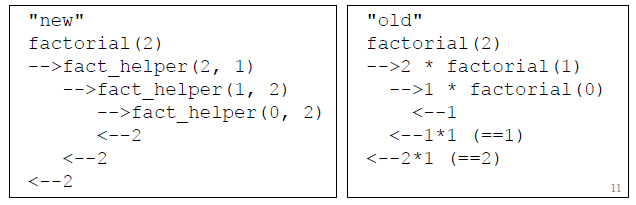
\includegraphics[scale=0.7]{sections/lec3/fact.png}	
	\end{center}

	\item Effects of the new version on the stack:
	\begin{itemize}
		\item The activation record of a function is needed only as long as there is computation left over and can be discarded as soon as the return value is known.
		\item With the new version, the concrete return value isn’t known at the time of the recursive call. However, we do know that whatever that recursive call returns, that will be our return value too.
		\item This means that the caller's stack frame isn't needed any more, and we can throw it away.
	\end{itemize}

	\item This is called \textbf{tail recursion}.
	\item If the result of the recursive call is returned directly with no pending computation, it is tail-recursive. Otherwise, it’s ``plain'' recursion.
\end{itemize}
